\documentclass{article}

\usepackage{fullpage}
\usepackage{graphicx,color}
\usepackage{amssymb}
\usepackage{braket}
\usepackage{physics}
%%\usepackage{qcircuit}
\usepackage{tikz}
\usetikzlibrary{quantikz}
\usepackage[ backend=biber,citestyle=numeric-comp]{biblatex}
\addbibresource{cites.bib}
\ExecuteBibliographyOptions{sorting=nyt,maxbibnames=100,doi=false,isbn=false,url=false}

\newcommand{\cnot}{\textsf{cnot}}
\newcommand{\qket}[1]{\ket{\tilde{#1}}}
\newcommand{\preim}[2]{\{\cdot\stackrel{#1}{\longleftarrow}{#2}\}}
\newcommand{\finset}[1]{[\mathbf{#1}]}
\newcommand{\red}[1]{{\color{red}{#1}}}
\newcommand{\todo}[1]{\fbox{\begin{minipage}{25em}{\red{#1}}\end{minipage}}}

%%%%%%%%%%%%%%%%%%%%%%%%%%%%%%%%%%%%%%%%%%%%%%%%%%%%%%%%%%%%%%%%%%%%%%%%%%%%%%%%%%%%%%%%%%

\title{Symbolic Retrodictive Execution of Quantum Circuits}
\author{Jacques Carette \qquad Gerardo Ortiz \qquad Amr Sabry}
\begin{document}
\maketitle

\begin{abstract}
The quantum circuit model consists of two classes of gates: (i)
quantum counterparts to classical reversible gates (e.g., Toffoli
gates), and (ii) genuine quantum gates with no classical counterpart
(e.g., Hadamard and phase gates). We make the remarkable observation,
that, for a number of quantum algorithms, judicious reasoning about
the classical components, ignoring all the quantum gates, is
sufficient. Put differently, in those cases, the quantum gates serve
no fundamental purpose and are actually distracting from an underlying
efficient classical algorithm. The result relies on the ability to
symbolically execute circuits, especially in a retrodictive fashion,
i.e., by making partial observations at the output site and proceeding
backwards to infer the implied initial conditions.
\end{abstract}

%%%%%%%%%%%%%%%%%%%%%%%%%%%%%%%%%%%%%%%%%%%%%%%%%%%%%%%%%%%%%%%%%%%%%%%%%%%%%%%%%%%%%%%%%%
\section{Introduction}

Retrodictive: 

Normal quantum evolution: from present to future

Now what if I had partial knowledge about the future; what can you say
about the present? (And then about the rest of the unknown future)

Can this help flow of information, complexity, etc?

In some cases, partial knowledge about the future is enough to predict
the present accurately enough to then predict everything about the
future; in some cases it is not enough

Possibility that collapse of wave function is information flow back
from measured future to present unknown initial conditions and then
back to rest of wave that was not measured









Given finite sets $A$ and $B$, a function $f : A \rightarrow B$ and an
element $y \in B$, we define $\preim{f}{y}$, the pre-image of $y$
under $f$, as the set $\{ x \in A ~|~ f(x) = y \}$. For example, let
$A = B = \{0,1,\ldots,15\}$ and let $f(x) = 7^x \mod 15$, then the
collection of values that $f$ maps to 4, $\preim{f}{4}$, is the set
$\{ 2, 6, 10, 14 \}$.

\begin{center}
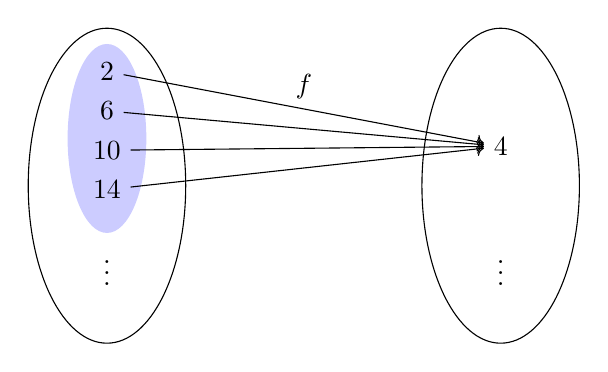
\begin{tikzpicture}
\draw (0,0) ellipse (1cm and 2cm);
\draw (5,0) circle (1cm and 2cm);
\fill[blue!20!white] (0,0.6) ellipse (0.5cm and 1.2cm);
\node (a) at (0,1.45) {2};
\node (b) at (0,0.95) {6};
\node (c) at (0,0.45) {10};
\node (d) at (0,-0.05) {14};
\node (t) at (5,0.5) {4};
\node at (0,-1) {$\vdots$};
\node at (5,-1) {$\vdots$};
\draw[->] (a) to node [above] {$f$} (t);
\draw[->] (b) -- (t);
\draw[->] (c) -- (t);
\draw[->] (d) -- (t);
\end{tikzpicture}
\end{center}

Finding the pre-image of a function is a mathematical question that
subsumes several practical computational problems such as pre-image
attacks on hash functions~\cite{10.1007/978-3-540-25937-4_24},
predicting environmental conditions that allow certain reactions to
take place in computational
biology~\cite{Klotz2013,akutsu2009analyses}, and finding the pre-image
of feature vectors in the space induced by a kernel in neural
networks~\cite{1353287}.

To appreciate the difficulty of computing pre-images in general, note
that SAT is a boolean function over the input variables and that
solving a SAT problem is asking for the pre-image of
\textsf{true}. Indeed, based on the conjectured existence of one-way
functions which itself implies $\mathit{P} \neq \mathit{NP}$, all
these pre-images calculations are believed to be computationally
intractable in their most general setting. What is however intriguing
is that many computational problems that have efficient quantum
algorithms are essentially queries over pre-images. We illustrate this
connection briefly in the remainder of this section and analyze it
further in the remainder of the paper.

Let $\finset{n}$ denote the finite set $\{ 0,1,\ldots,(n-1)\}$. The
parameter $n$ determines the problem size in all the problems below
(except Deutsch which is a fixed sized problem).

\paragraph*{Deutsch.}
The conventional statement of the problem is to determine if a
function $\finset{2} \rightarrow \finset{2}$ is constant or
balanced. An equivalent statement is to answer a query about the
cardinality of a pre-image. In this case, if the cardinality of the
pre-image of any value in the range is even i.e. 0 or 2, the function
must be constant and if it is odd, i.e., it contains just one element,
the function must be balanced.

\paragraph*{Deutsch-Jozsa.}
The problem is a generalization of the previous one: the question is
to determine if a function $\finset{2^n} \rightarrow \finset{2}$ for
some $n$ is constant or balanced. When expressed as a pre-image
computation, the problem reduces to a query distinguishing the
following three situations about the pre-image of a value in the range
of the function: is the cardinality of the pre-image equal to 0,
$2^n$, or $2^{n-1}$? In the first two cases, the function is constant
and in the last case, the pre-image contains half the values in the
domain indicating that the function is balanced.

\paragraph*{Bernstein-Vazirani.}
We are given a function $f : \finset{2^n} \rightarrow \finset{2}$
that hides a secret number $s \in \finset{2^n}$. We are promised the
function is defined using the binary representations $\sum_i^{n-1}
x_i$ and $\sum_i^{n-1} s_i$ of $x$ and $s$ respectively as follows:
\[
f(x) = \sum_{i=0}^{n-1} s_ix_i \mod{2}
\]
The goal is to determine the secret number $s$. 

Expressing the problem as a pre-image calculation is slightly more
involved than in the previous two cases. To determine $s$, we make $n$
queries to the pre-image of a value in the range of the
function. Query $i$ asks whether $2^i$ is a member of the pre-image
and the answer determines bit $i$ of the secret $s$. Indeed, by
definition, $f(2^i) = s_i$ and hence $s_i$ is 1 iff $2^i$ is a member
of the pre-image of 1.

\paragraph*{Simon.}
We are given a 2-1 function $f : \finset{2^n} \rightarrow
\finset{2^n}$ with the property that there exists an $a$ such $f(x) =
f(x \oplus a)$ for all~$x$; the goal is to determine $a$. When
expressed as a computation of pre-images, the problem statement
becomes the following. Pick an arbitrary $x$ and compute the pre-image
of $f(x)$. It must contain exactly two values one of which is $x$. The
problem then reduces to finding the other value in the pre-image.

\paragraph*{Shor.}
The quantum core of the algorithm is the following. We are given a
periodic function $f(x) = a^x \mod{2^n}$ and the goal is to determine
the period. As a computation over pre-images, the problem can be
recast as follows. For an arbitrary $x$, compute the pre-image of
$f(x)$ and query it to determine the period.

%%%%%%%%%%%%%%%%%%%%%%%%%%%%%%%%%%%%%%%%%%%%%%%%%%%%%%%%%%%%%%%%%%%%%%%%%%%%%%%%%%%%%%%%%%
\section{The Quantum Approach}

A brute force solution to all the problems in the previous section is
straightforward: try every value in the domain of the relevant
function to calculate the required pre-image. Then, given complete
knowledge of the pre-image, all the needed queries can be easily
answered. This approach is, of course, not practical, as it is
exponential in the problem size $n$. Furthermore, even if some
shortcuts were discovered to speed up the calculation of the
pre-image, there is the additional non-trivial requirement of
performing efficient queries on the pre-image.

Luckily, the problems of concern to us are quite special: (i) the
functions are not arbitrary but have additional structure that can be
exploited, and (ii) we never need access to all the elements in the
pre-image; we just need to answer aggregate queries about the
pre-images. Quantum algorithms somehow exploit these properties along
with some physical principles to solve these problems efficiently. To
understand the precise way in which this is happening, we start with
the template of the quantum circuit used for solving all the problems
above in Fig.~\ref{fig:templateQC}.

\begin{figure}[t]
\begin{center}
\begin{quantikz}[slice all,row sep=0.7cm,column sep=1cm]
   \lstick{$\ket{0}^{\otimes n}$} &[3em] 
   \gate{H^{\otimes n}}\qwbundle{n} & 
   \gate[wires=2][2cm]{U_f}\gateinput{$x$}\gateoutput{$x$} &
   \qw &
   \gate{\mathit{QFT}} &
   \meter{} & 
   \rstick{$\tilde{v}$}\cw
   \\
   \lstick{$\displaystyle{\frac{1}{\sqrt{2^m}}\sum_{y=0}^{2^m-1} \alpha_y\ket{y}}$} &[3em]
   \qw\qwbundle{m} &
   \gateinput{$y$}\gateoutput{$f(x)\oplus y$} &
   \meter{} &
   \rstick{$w$}\cw 
\end{quantikz}
\end{center}
\caption{\label{fig:templateQC}Template quantum circuit}
\end{figure}

The core of the circuit is the $U_f$ block which can be assumed to be
implemented using only generalized Toffoli gates. The block implements
the unitary transformation: $U_f(\ket{x}\ket{y}) = \ket{x}\ket{f(x)
  \oplus y}$ where $\oplus$ is the (bitwise) exclusive-or operation;
it defines the function of interest whose pre-image properties are to
be calculated. The inputs of the $U_f$ block are grouped in two
registers: the top register contains an equal superposition of all
possible inputs to $f$; the second register is prepared in initial
states that depend on the specific algorithm. Thus, the state at slice
(1) in the figure is:
  \[
  \frac{1}{\sqrt{2^n}\sqrt{2^m}}\sum_{x=0}^{2^n-1} ~\sum_{y=0}^{2^m-1} ~\ket{x}\ket{y}
  \]
This is transformed by $U_f$ to:
  \[
  \frac{1}{\sqrt{2^n}\sqrt{2^m}}
  \sum_{x=0}^{2^n-1} ~\sum_{y=0}^{2^m-1} ~\ket{x}\ket{f(x)\oplus y}
  \]
So far, nothing too interesting is happening: we have just produced a
superposition of states where each state is a possible input to $f$,
say $x$, tensored with $f(x) \oplus y$, the result of applying $f$ to
this particular input adjusted by the second register $y$. At slice
(3), something remarkable occurs; the result $w$ of measuring the
second register ``kicks back'' information to the first register whose
state becomes a superposition of those values $x$ that are consistent
with the measurement, i.e., \emph{the pre-image of $w$ under $f$!}
That pre-image representation is then analyzed using the Quantum
Fourier Transform (QFT) to produce the final result.

To make the previous discussion more concrete, we show the full
execution of the quantum algorithm on a few examples.

%%%
\subsection{Bernstein-Vazirani}

\begin{figure}[t]
\begin{center}
\begin{quantikz}[row sep=0.2cm,column sep=1cm]\label{eq:bernstein-vazirani}
   \lstick{$\ket{0}$} & \gate{H}\slice{1} & \qw      & \qw      & \qw       & \qw \slice{2}      & \qw\slice{3} & \gate{H} 
   & \meter{} & \rstick{$\tilde{v_0}$}\cw \\
   \lstick{$\ket{0}$} & \gate{H} & \ctrl{7} & \qw      & \qw       & \qw       & \qw & \gate{H} 
   & \meter{} & \rstick{$\tilde{v_1}$}\cw \\
   \lstick{$\ket{0}$} & \gate{H} & \qw      & \qw      & \qw       & \qw       & \qw & \gate{H} 
   & \meter{} & \rstick{$\tilde{v_2}$}\cw \\
   \lstick{$\ket{0}$} & \gate{H} & \qw      & \ctrl{5} & \qw       & \qw       & \qw & \gate{H} 
   & \meter{} & \rstick{$\tilde{v_3}$}\cw \\
   \lstick{$\ket{0}$} & \gate{H} & \qw      & \qw      & \ctrl{4}  & \qw       & \qw & \gate{H} 
   & \meter{} & \rstick{$\tilde{v_4}$}\cw \\
   \lstick{$\ket{0}$} & \gate{H} & \qw      & \qw      & \qw       & \ctrl{3}  & \qw & \gate{H} 
   & \meter{} & \rstick{$\tilde{v_5}$}\cw \\
   \lstick{$\ket{0}$} & \gate{H} & \qw      & \qw      & \qw       & \qw       & \qw & \gate{H} 
   & \meter{} & \rstick{$\tilde{v_6}$}\cw \\
   \lstick{$\ket{0}$} & \gate{H} & \qw      & \qw      & \qw       & \qw       & \qw & \gate{H} 
   & \meter{} & \rstick{$\tilde{v_7}$}\cw \\
   \lstick{$\ket{1}$}  & \gate{H}  & \targ{}  & \targ{}  & \targ{}   & \targ{}   & \meter{} 
   & \rstick{$w$}\cw
\end{quantikz}
\end{center}
\caption{\label{fig:bv}Example Circuit for Bernstein-Vazirani Algorithm}
\end{figure}

The circuit in Fig.~\ref{fig:bv} solves the problem for $n=8$ and a
hidden number 92 ($= 00111010$ in binary notation). As required, the
circuit between slice (1) and slice (2), collects the sum of the $x_i$
at positions that match the occurrences of 1 in the secret string. The
evolution proceeds as follows. At slice (1), the top 8 qubits are each
in the state $\ket{+}$ and the bottom qubit is in the state $\ket{-}$,
i.e., the state is $(1/3)~\ket{++++++++-}$. In the evolution between
slices (1) and (2), qubits 0, 2, 6, and 7 are untouched and remain in
the state $\ket{+}$. Each of the other four qubits becomes $\ket{-}$
as the phase of the target qubit is kicked back to the control qubit
by the \cnot\  operation. The full state at slice (2) is
$(1/3)~\ket{+-+---++-}$. At this point, we perform a measurement on
the bottom qubit which returns 0 or 1 with equal probability. This
measurement causes collapses the top 8 qubits to $\pm
(1/2\sqrt{2})~\ket{+-+---++}$. After applying all the Hadamard gates,
the measurement is deterministically $\ket{01011100}$ with the most
significant bit at the right. This is the secret number. 

Instead of this execution model, we now explore an alternative
execution that starts from the observation $w$ and proceeds from slice
(2) back towards slice (1) collecting the information necessary to
answer the required pre-image query. As explained in the previous
section, the secret number can be reconstructed once we know, for each
$i$, whether the number $2^i$ is a member of the pre-image. When
expressed in terms of bits, this means that we need to know, for each
bit position $i$, whether the corresponding qubit contributes to the
definition of the pre-image. We therefore start a backwards execution
starting with the state $\ket{x_0x_1x_2x_3x_4x_5x_6x_7F()}$ where
$F()$ expresses that the last qubit has not been shown to depend on
any qubit so far and the $x_i$ symbols are placeholders for unknown
values. We trace the execution symbolically:
\[\begin{array}{rcl}
\ket{x_0x_1x_2x_3x_4x_5x_6x_7F()} &\leftarrow& \ket{x_0x_1x_2x_3x_4x_5x_6x_7F(x_5)} \\
&\leftarrow& \ket{x_0x_1x_2x_3x_4x_5x_6x_7F(x_4,x_5)} \\
&\leftarrow& \ket{x_0x_1x_2x_3x_4x_5x_6x_7F(x_3,x_4,x_5)} \\
&\leftarrow& \ket{x_0x_1x_2x_3x_4x_5x_6x_7F(x_1,x_3,x_4,x_5)}
\end{array}\]
For each operation $\cnot(x,v)$, we add $x$ to the list of variables
on which $v$ depends. At the end of the execution, we conclude that
$x_1$, $x_3$, $x_4$, and $x_5$ are the relevant qubits, from which we
infer that the secret string must be $00111010$.

%%%
\subsection{E1}

\begin{figure}[t]
    \centering
    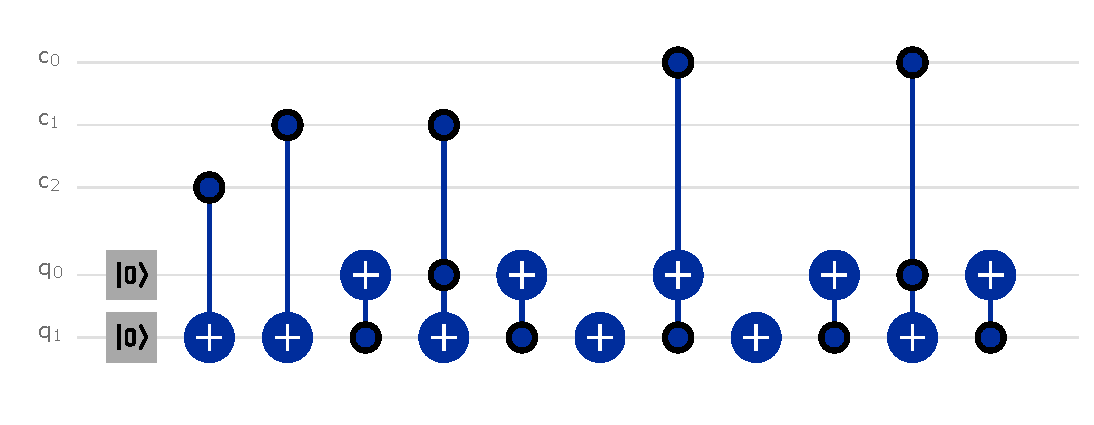
\includegraphics[scale=0.7]{factor.pdf}
    \caption{An Optimized Circuit for $U_f$ where $f(x) = 4^x \mod{21}$}
    \label{fig:factor}
\end{figure}


Consider the small circuit in Fig.~\ref{fig:factor}. The scenario we
are investigating is the following. The initial state of $c_2,c_1,c_0$
is unknown but both the initial state and final state of $q_1,q_0$ are
known. The initial state is clearly $00$ and let's assume for the
remaining of this example that the final state is $01$. The question
is what can we infer about $c_2,c_1,c_0$? To answer the question, we
will symbolically evaluate the circuit starting from the final state
$c_0,c_1,c_2,1,0$ and going backwards towards the initial state as
shown in Fig.~\ref{fig:deriv}. In step (1), we encounter a \texttt{cx}
acting on $q_1$ and $q_0$ which are known. In step (2), we are not so
lucky: we encounter a \texttt{ccx} gate with one unknown control wire
but all hope is not lost. The action of $\texttt{ccx}~a~b~c$ is to
update $c$ to be $a \wedge b \oplus c$ where $\wedge$ is boolean
conjunction (often omitted when clear from context) and $\oplus$ is
the exclusive-or operation. In step (2), this means that the target
wire $q_1$ should be updated to $1 \wedge c_0 \oplus 0$ which
simplifies to $c_0$.

At the end of the retrodictive execution, we conclude that $q_0 = 1
\oplus c_0 \oplus c_1$ and $q_1 = c_0 \oplus c_2$ which needs to
reconciled with the initial condition that $q_0 = q_1 = 0$. Solving
these equations gives two possible solutions for $c_2j,c_1,c_0$:
either $c_2,c_1,c_0 = 010$ or $c_2,c_1,c_0 = 101$.

Another perspective on this analysis is the following. Assume
$c_2,c_1,c_0$ started in an equal superposition and that $q_1,q_0$
were measured to be $01$ after applying the circuit to the incoming
superposition. The measurement of $q_1q_0$ would essentially cause a
\emph{phase kickback} collapsing the equal superposition of all
possible values of $c_2,c_1,c_0$ to just the two possible values that
are consistent with the measurement.

\begin{figure}[t]
\[\begin{array}{lclr}
&& c_0~c_1~c_2~(q_0=1)~(q_1=0) & (0) \\
(\texttt{cx}~q_1~q_0)      \\ && c_0~c_1~c_2~(q_0=1)~(q_1=0) & (1) \\
(\texttt{ccx}~c_0~q_0~q_1) \\ && c_0~c_1~c_2~(q_0=1)~(q_1=c_0) & (2) \\
(\texttt{cx}~q_1~q_0)      \\ && c_0~c_1~c_2~(q_0=1 \oplus c_0)~(q_1=c_0) & (3) \\
(\texttt{x}~q_1)           \\ && c_0~c_1~c_2~(q_0=1 \oplus c_0)~(q_1=1 \oplus c_0) & (4) \\
(\texttt{ccx}~c_0~q_1~q_0) \\ && c_0~c_1~c_2~(q_0=1 \oplus c_0)~(q_1=1 \oplus c_0) & (5) \\
(\texttt{x}~q_1)           \\ && c_0~c_1~c_2~(q_0=1 \oplus c_0)~(q_1=c_0) & (6) \\
(\texttt{cx}~q_1~q_0)      \\ && c_0~c_1~c_2~(q_0=1)~(q_1=c_0) & (7) \\
(\texttt{ccx}~c_1~q_0~q_1) \\ && c_0~c_1~c_2~(q_0=1)~(q_1=c_0 \oplus c_1) & (8) \\
(\texttt{cx}~q_1~q_0)      \\ && c_0~c_1~c_2~(q_0=1 \oplus c_0 \oplus c_1)~(q_1=c_0 \oplus c_1) & (9) \\
(\texttt{cx}~c_1~q_1)      \\ && c_0~c_1~c_2~(q_0=1 \oplus c_0 \oplus c_1)~(q_1=c_0) & (10) \\
(\texttt{cx}~c_2~q_1)      \\ && c_0~c_1~c_2~(q_0=1 \oplus c_0 \oplus c_1)~(q_1=c_0 \oplus c_2) & (11)
\end{array}\]
\caption{Retrodictive execution of the circuit in Fig.~\ref{fig:factor}}
\label{fig:deriv}
\end{figure}

%%%
\subsection{E2}

\begin{figure}[t]
    \centering
    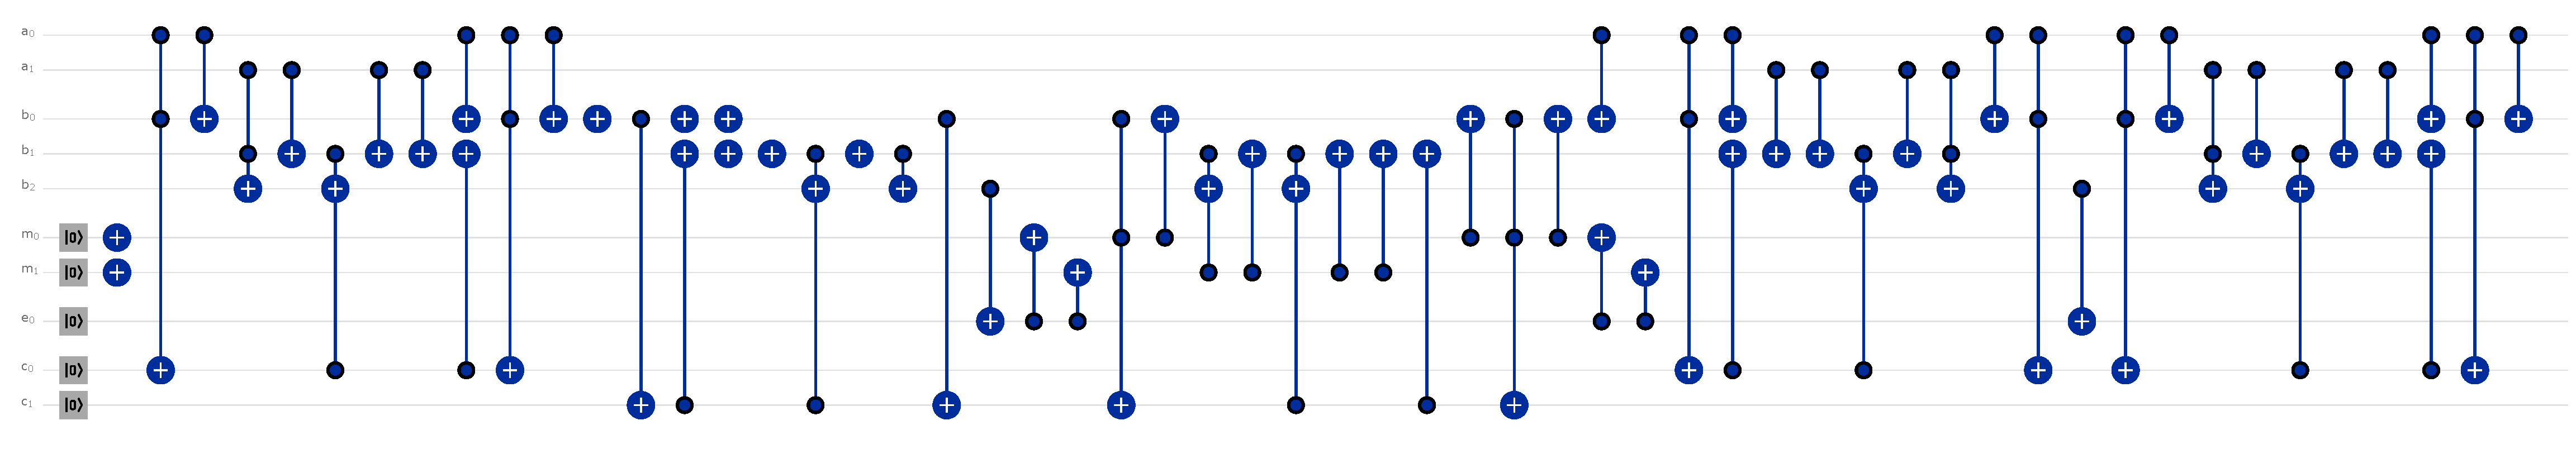
\includegraphics[scale=0.2]{adder.pdf}
    \caption{A Circuit for 2-bit Carry Adder}
    \label{fig:adder}
\end{figure}

Fig.~\ref{fig:adder} shows a larger circuit. The top five wires are
the interesting inputs while the bottom five wires serve as ancilla
bits initialized to fixed values. The question we are interested in
this case is the following: say we learn that at the end of the
execution we have $b_2b_1b_0 = 001$, what possible input values for
$a_1a_0$ and $b_2b_1b_0$ could have produced such a result? Using the
same process as above, we calculate $b_0 = 1 \oplus a_0 \oplus a_1$,
$b_1 = a_1 \oplus a_0a_1$, and $b_2 = 0$.

%%
\subsection{Perspective}

Quantum algorithms typically operate on a \emph{black box} holding a
classical function whose properties need to be computed. The general
structure of these algorithms is to (i) create a superposition of
values to be passed as inputs to the black box, (ii) apply the
operation inside the black box, and (iii) post-process the output of
the black box. We observe that, in quite a few cases, steps (i) and
(iii) are actually unnecessary and that the entire ``quantum''
algorithm can be executed by forward or backward, full or partial,
efficient classical \emph{symbolic execution} of the black box.


typical use: superposition, Uf, measure second register; we only care
about which x has f(x) = r

By default all functions are reversible. 

To make them irreversible you fix h and delete g. If you delete too
much the function becomes very expensive to reverse. So one way
functions emerge


simplify function has polynomial realization and we want
statistics about the kernel (not necessarily compute it exactly)



collect assumptions:


important that no matter what measurement we ddo on w, propery we want is the same


since we say that algos relatedd to preimages lets do naive thing and eval backwards

assumptions we have a rev ccircuit efficient forward
two inputs: first is full superposition; second whatever
first output same as first input; but that is only at point 2; at point 3 explain kick bacck; misleadding to think it is the same after 3
second output is result of functionn; measure; have element of range; go bacck with that elem
if we knew first output as well as w then eval backwards same compleity but we only know w and we don't know first output; because we are starting at 3 not 2

we have no use for H block; it was only there for the forward execc to express our ccomlete ignorance o fthe future; prepared with every x but if we have knowledge about future (w measured) we go backc to find the values of x in the present that would db consistent with w so general circuit redduces to :

...

fix picc to have amplitudes with y (most general)

To what extent are the quantum algorithms above taking advantage of
non-classical features. We posit that pre-image computation can be, at
least for some of the some of the algorithms, be performed
classically. The main insight needed for that is to perform the
execution \emph{symbolically}. We illustrate the idea with two
examples.


%%%

%%%%%%%%%%%%%%%%%%%%%%%%%%%%%%%%%%%%%%%%%%%%%%%%%%%%%%%%%%%%%%%%%%%%%%%%%%%%%%%%%%%%%%%%%%
\section{Two Small Factoring Problems}

%%%
\subsection{Factoring 15}

\begin{figure}[t]
\begin{center}
\begin{quantikz}[row sep=0.2cm,column sep=1cm]
\lstick{$x_2 = \ket{0}$} & \gate{H}\slice{1} & \qw & \qw \slice{2}
      & \qw\slice{3} & \gate[wires=3][1cm]{QFT} & \meter{} & \rstick{$\tilde{v_2}$}\cw \\
\lstick{$x_1 = \ket{0}$} & \gate{H} & \qw & \qw       
      & \qw & & \meter{} & \rstick{$\tilde{v_1}$}\cw \\
\lstick{$x_0 = \ket{0}$} & \gate{H} & \octrl{3} & \ctrl{1}
      & \qw & & \meter{} & \rstick{$\tilde{v_0}$}\cw \\
\lstick{$\ket{0}$} & \qw & \qw & \targ{}
      & \meter{} & \rstick{$\tilde{e_2}$}\cw \\
\lstick{$\ket{0}$} & \qw & \qw  & \qw
      & \meter{} & \rstick{$\tilde{e_1}$}\cw \\
\lstick{$\ket{0}$} & \qw & \targ{} & \qw 
      & \meter{} & \rstick{$\tilde{e_0}$}\cw 
\end{quantikz}
\end{center}
\caption{\label{fig:shor15}Finding the period of $4^x \mod{15}$}
\end{figure}

\[\begin{array}{rcl}
(1/\sqrt{6})~\ket{+++000}
  &=& (1/\sqrt{12})~(\ket{++0000} + \ket{++1000}) \\
  &\rightarrow& (1/\sqrt{12})~(\ket{++1000} + \ket{++0000}) \\
  &\rightarrow& (1/\sqrt{12})~(\ket{++1001} + \ket{++0000}) \\
  &\rightarrow& (1/\sqrt{12})~(\ket{++0001} + \ket{++1000}) \\
  &\rightarrow& (1/\sqrt{12})~(\ket{++0001} + \ket{++1100}) 
\end{array}\]
Say we measure $001$ in the second register. The state of the first
register collpases to $(1/\sqrt{3})~\ket{++0}$ which is given to the
QFT block. The QFT result is $(1/\sqrt{2})~(\qket{000} +
\qket{100})$. If measure 0 we repeat the experiment. If we measure 4
we infer that the period is 8/4 = 2 and hence that the factors are 3
and 5.

Now do retrodictive execution starting with $\ket{x_2x_1x_0001}$:
\[\begin{array}{rcl}
\ket{x_2x_1x_0001}
  &\rightarrow& \ket{x_2x_1x_0x_001} \\
  &\rightarrow& \ket{x_2x_1\overline{x_0}x_001} \\
  &\rightarrow& \ket{x_2x_1\overline{x_0}x_00x_0} \\
  &\rightarrow& \ket{x_2x_1x_0x_00x_0} 
\end{array}\]
Initial condition says $x_0 = 0$ and hence the pre-image is $? ? 0$
which matches $000, 010, 100, 110$, i.e., the period is 2.

%%%
\subsection{Factoring 21}

\begin{figure}[t]
\begin{center}
\begin{quantikz}[row sep=0.1cm,column sep=0.1cm]
\lstick{$x_3 = \ket{0}$} & \gate{H}\slice{1} & \octrl{8} & \octrl{8} & \ctrl{8} &
  \octrl{5} & \octrl{7} & \octrl{8} &   
  \octrl{5} & \octrl{7} & \octrl{8} &
  \ctrl{5} & \ctrl{7} & \ctrl{8}\slice{} &   
  \octrl{4} & \ctrl{4} & \ctrl{4} &   
  \octrl{5} & \ctrl{5} & \ctrl{5} &
  \octrl{6} & \ctrl{6} & \octrl{7} & \ctrl{7} &
  \qw \slice{2} & \qw\slice{3} & \gate[wires=4][1cm]{QFT} & 
  \meter{} & \rstick{$\tilde{v_3}$}\cw \\
\lstick{$x_2 = \ket{0}$} & \gate{H} & \octrl{7} & \ctrl{7} & \ctrl{7} & 
  \octrl{4} & \octrl{6} & \octrl{7} &   
  \ctrl{4} & \ctrl{6} & \ctrl{7} &   
  \ctrl{4} & \ctrl{6} & \ctrl{7} &   
  \octrl{3} & \octrl{3} & \ctrl{3} &   
  \octrl{4} & \octrl{4} & \ctrl{4} &
  \ctrl{5} & \octrl{5} & \ctrl{6} & \octrl{6} &
  \qw & \qw & & \meter{} & \rstick{$\tilde{v_2}$}\cw \\
\lstick{$x_1 = \ket{0}$} & \gate{H} & \octrl{6} & \ctrl{6} & \octrl{6} & 
  \octrl{3} & \octrl{5} & \octrl{6} &   
  \ctrl{3} & \ctrl{5} & \ctrl{6} &   
  \octrl{3} & \octrl{5} & \octrl{6} &   
  \ctrl{2} & \octrl{2} & \ctrl{2} &   
  \ctrl{3} & \octrl{3} & \ctrl{3} &
  \octrl{4} & \ctrl{4} & \octrl{5} & \ctrl{5} &
  \qw & \qw & & \meter{} & \rstick{$\tilde{v_1}$}\cw \\
\lstick{$x_0 = \ket{0}$} & \gate{H} & \octrl{5} & \octrl{5}  & \octrl{5} & 
  \ctrl{2} & \ctrl{4} & \ctrl{5} &   
  \ctrl{2} & \ctrl{4} & \ctrl{5} &   
  \ctrl{2} & \ctrl{4} & \ctrl{5} &   
  \octrl{1} & \octrl{1} & \octrl{1} &   
  \ctrl{2} & \ctrl{2} & \ctrl{2} &
  \octrl{3} & \octrl{3} & \ctrl{3} & \ctrl{3} &
  \qw & \qw & & \meter{} & \rstick{$\tilde{v_0}$}\cw \\
\lstick{$\ket{0}$} & \qw & \qw & \qw & \qw &
  \qw & \qw & \qw &     
  \qw & \qw & \qw &     
  \qw & \qw & \qw &     
  \targ{} & \targ{} & \targ{} &     
  \qw & \qw & \qw &     
  \qw & \qw & \qw & \qw & 
  \qw & \meter{} & \rstick{$\tilde{e_4}$}\cw \\
\lstick{$\ket{0}$} & \qw & \qw & \qw & \qw & 
  \targ{} & \qw & \qw &     
  \targ{} & \qw & \qw & 
  \targ{} & \qw & \qw &     
  \qw & \qw & \qw &     
  \targ{} & \targ{} & \targ{} &     
  \qw & \qw & \qw & \qw & 
  \qw & \meter{} & \rstick{$\tilde{e_3}$}\cw \\
\lstick{$\ket{0}$} & \qw & \qw & \qw & \qw & 
  \qw & \qw & \qw &     
  \qw & \qw & \qw &     
  \qw & \qw & \qw &     
  \qw & \qw & \qw &     
  \qw & \qw & \qw &     
  \targ{} & \targ{} & \qw & \qw & 
  \qw & \meter{} & \rstick{$\tilde{e_2}$}\cw \\
\lstick{$\ket{0}$} & \qw & \qw & \qw & \qw &
  \qw & \targ{}& \qw &     
  \qw & \targ{} & \qw &     
  \qw & \targ{} & \qw &     
  \qw & \qw & \qw &     
  \qw & \qw & \qw &     
  \qw & \qw & \targ{} & \targ{} & 
  \qw & \meter{} & \rstick{$\tilde{e_1}$}\cw \\
\lstick{$\ket{0}$} & \qw & \targ{} & \targ{} & \targ{} & 
  \qw & \qw & \targ{} &     
  \qw & \qw & \targ{} &     
  \qw & \qw & \targ{} &     
  \qw & \qw & \qw &     
  \qw & \qw & \qw &     
  \qw & \qw & \qw & \qw & 
  \qw & \meter{} & \rstick{$\tilde{e_0}$}\cw 
\end{quantikz}
\end{center}
\caption{\label{fig:shor21}Finding the period of $11^x \mod{21}$}
\end{figure}

\[\begin{array}{rcl}
&&   \ket{0000}\ket{00000} +
     \ket{0001}\ket{00000} +
     \ket{0010}\ket{00000} +
     \ket{0011}\ket{00000} + \\
&&     \ket{0100}\ket{00000} + 
     \ket{0101}\ket{00000} +
     \ket{0110}\ket{00000} +
     \ket{0111}\ket{00000} + \\
&&     \ket{1000}\ket{00000} +
     \ket{1001}\ket{00000} + 
     \ket{1010}\ket{00000} +
     \ket{1011}\ket{00000} + \\
&&     \ket{1100}\ket{00000} +
     \ket{1101}\ket{00000} +
     \ket{1110}\ket{00000} +
     \ket{1111}\ket{00000} \\[2em]
&\rightarrow&
     \ket{0000}\ket{00001} +
     \ket{0001}\ket{01011} +
     \ket{0010}\ket{00000} +
     \ket{0011}\ket{00000} + \\
&&     \ket{0100}\ket{00000} + 
     \ket{0101}\ket{00000} +
     \ket{0110}\ket{00001} +
     \ket{0111}\ket{01011} + \\
&&     \ket{1000}\ket{00000} +
     \ket{1001}\ket{00000} + 
     \ket{1010}\ket{00000} +
     \ket{1011}\ket{00000} + \\
&&     \ket{1100}\ket{00001} +
     \ket{1101}\ket{01011} +
     \ket{1110}\ket{00000} +
     \ket{1111}\ket{00000} \\[2em]
&\rightarrow&
     \ket{0000}\ket{00001} +
     \ket{0001}\ket{01011} +
     \ket{0010}\ket{10000} +
     \ket{0011}\ket{01000} + \\
&&     \ket{0100}\ket{00100} + 
     \ket{0101}\ket{00010} +
     \ket{0110}\ket{00001} +
     \ket{0111}\ket{01011} + \\
&&     \ket{1000}\ket{10000} +
     \ket{1001}\ket{01000} + 
     \ket{1010}\ket{00010} +
     \ket{1011}\ket{00010} + \\
&&     \ket{1100}\ket{00001} +
     \ket{1101}\ket{01011} +
     \ket{1110}\ket{10000} +
     \ket{1111}\ket{01000} \\[2em]
&\rightarrow&
     (\ket{0000}+\ket{0110}+\ket{1100})\ket{00001} + \\
&&   (\ket{0101}+\ket{1011})\ket{00010} + \\
&&   (\ket{0100}+\ket{1010})\ket{00100} + \\
&&   (\ket{0011}+\ket{1001}+\ket{1111})\ket{01000} + \\
&&   (\ket{0001}+\ket{0111}+\ket{1101})\ket{01011} + \\
&&   (\ket{0010}+\ket{1000}+\ket{1110})\ket{10000} 
\end{array}\]
Say we measure $01011$ in second register, the state collapses to
$\ket{0001}+\ket{0111}+\ket{1101}$. QFT probabilities are:
\[\begin{array}{rcl}
\qket{0} &:& 19\% \\
\qket{8} &:& 19\% \\
\qket{3} &:& 12\% \\
\qket{5} &:& 12\% \\
\qket{11} &:& 12\% \\
\qket{13} &:& 12\% \\
\qket{2} &:& 2\% \\
\qket{4} &:& 2\% \\
\qket{6} &:& 2\% \\
\qket{10} &:& 2\% \\
\qket{12} &:& 2\% \\
\qket{14} &:& 2\% 
\end{array}\]

Continued fraction: measure 8, should be close to m16/r, gives us r=2 bad

measure 3; should be close to m16/r; gives us r = 5; odd bad
measure 5; bad
measure 11

gcd 10 21
\begin{verbatim}
m16/r ~ 11

11/16 ~ m/r

11/16 = 1/(1+5/11) = 1/(1+(1/2+1/5))


\end{verbatim}

%%%%%%%%%%%%%%%%%%%%%%%%%%%%%%%%%%%%%%%%%%%%%%%%%%%%%%%%%%%%%%%%%%%%%%%%%%%%%%%%%%%%%%%%%%
%%%%%%%%%%%%%%%%%%%%%%%%%%%%%%%%%%%%%%%%%%%%%%%%%%%%%%%%%%%%%%%%%%%%%%%%%%%%%%%%%%%%%%%%%%

\printbibliography
\end{document}

%%%%%%%%%%%%%%%%%%%%%%%%%%%%%%%%%%%%%%%%%%%%%%%%%%%%%%%%%%%%%%%%%%%%%%%%%%%%%%%%%%%%%%%%%%
\section{Retrodictive}

\subsection{Retrodictive Classical Computation}

Were we lucky in these two examples or is there something interesting happening; we can use ideas from physics that are not all quantum to try to improve classical computation

We need to explain ideas about time-reversal, prediction and retrodiction in 
physics. The laws of computation and the laws of physics are intimately related. 
When does knowing something about the future help us unveil the structure or 
symmetries of the past? It is like a detective story, but one with 
ramifications in complexity and/or efficiency. Problems involving questions 
where answers demand a Many(past)-to-one(future) map are at the root of 
our proposal.... {\color{red} Difference between exploiting or not entanglement
in the unitary evolution.}

As we demonstrate, the family of quantum algorithms initiated by
Deutsch's algorithm and culminating with Shor's algorithm (i) solves
variants of the pre-image problem efficiently, and, in that context,
(ii) answering queries about pre-images is closely related to
\emph{retrodictive quantum theory}~\cite{sym13040586},
retrocausality~\cite{Aharonov2008}, and the time-symmetry of physical
laws~\cite{RevModPhys.27.179}.


\begin{itemize}
\item Retrodictive execution more efficient in some cases. What cases?
\item Here are three examples: Deutsch-Jozsa, Simon, Shor when period
  is close to a power of 2
\item Symbolic (retrodictive) evaluation as a broader perspective to classical computation
\item Symbolic execution allows you to express/discover interference via shared variables
\item When interference pattern is simple symbolic execution reveals
  solutions faster (and completely classically)
\item Symbolic execution as a “classical waves” computing paradigm
\end{itemize}


to represent unequal superpositions do multiple runs with vars the
first has x1 x2 etc the second has y1 2y2 etc or y2/2 etc, or with
various patterns of negative weights.... And then the punchline would
be to interpret the negative backwards. So instead of all forward or
all retro we have some values going forward and then backwards

Start with the story about function many to one etc why superpositions
because we don’t know which values so we try all easy to represent by
unknown vars so we can represent superpositions as vars and equations
between them but at the end we want stats about superpositions slow
way is to generate all equations and solve faster way is generate many
sets of equations with different weights and sum to get your stats

%%%
\subsection{Deutsch}

The problem is to determine if a function $\finset{2} \rightarrow
\finset{2}$ is constant or balanced. The only relevant part of the circuit is:

\bigskip
\begin{center}
\begin{quantikz}\label{eq:deutsch}
   \lstick{$x$} & \gate[wires=2][1.5cm]{U_f} & \rstick{$x$} \qw \\
   \lstick{$y$} & \qw        & \rstick{$\ket{0}$} \qw
\end{quantikz}
\end{center}
\medskip 

 We fix the ancillary output to a possible boundary condition, say
 $\ket{0}$, and perform a retrodictive execution of the circuit. This
 execution produces a formula for $y$ that depends on the function $f$
 in the black box. When the function $f$ is a constant function, the
 formula is the corresponding constant $0$ or $1$. When the function
 is balanced the resulting formula is $x$ (when the function is the
 identity) or $1+x$ (when the function is boolean negation).

%%%
\subsection{Deutsch-Jozsa}

The problem is a generalization of the previous one: the question is
to determine if a function $\mathbb{B}^n \rightarrow \mathbb{B}$ is
constant or balanced. The circuit is identical to above except that
$x$ is now a collection of qubits:

\begin{quantikz}\label{eq:deutsch-jozsa}
   \lstick{$x_0$}     & \gate[wires=4][1.5cm]{U_f} & \rstick{$x_0$}     \qw \\
   \lstick{$x_1$}     & \ghost{U_f}        & \rstick{$x_1$}     \qw \\
   \lstick{$\ldots$}  & \ghost{U_f}        & \rstick{$\ldots$}  \qw \\
   \lstick{$x_{{n-1}}$} & \ghost{U_f}        & \rstick{$x_{{n-1}}$} \qw \\
   \lstick{$y$}       & \ghost{U_f}        & \rstick{$\ket{0}$} \qw
\end{quantikz}
\medskip 

Again, we fix the ancillary output to a possible boundary condition,
say $\ket{0}$, and perform a retrodictive execution of the
circuit. This execution produces a formula for $y$ that depends on the
function $f$ in the black box. When the function $f$ is a constant
function, the formula is the corresponding constant $0$ or $1$. When
the function is balanced the resulting formula involves at least one
variable $x_i$.

%%%
\subsection{Bernstein-Vazirani}

The circuit below gives the definition of the oracle $U_f$ for an
instance of the problem where $n=8$ and the hidden number $s$ is
$00111010$:

\bigskip
\begin{center}
\begin{quantikz}\label{eq:bernstein-vazirani}
   \lstick{$x_0$} & \qw      & \qw      & \qw       & \qw       & \rstick{$x_0$}     \qw \\
   \lstick{$x_1$} & \ctrl{7} & \qw      & \qw       & \qw       & \rstick{$x_1$}     \qw \\
   \lstick{$x_2$} & \qw      & \qw      & \qw       & \qw       & \rstick{$x_2$}     \qw \\
   \lstick{$x_3$} & \qw      & \ctrl{5} & \qw       & \qw       & \rstick{$x_3$}     \qw \\
   \lstick{$x_4$} & \qw      & \qw      & \ctrl{4}  & \qw       & \rstick{$x_4$}     \qw \\
   \lstick{$x_5$} & \qw      & \qw      & \qw       & \ctrl{3}  & \rstick{$x_5$}     \qw \\
   \lstick{$x_6$} & \qw      & \qw      & \qw       & \qw       & \rstick{$x_6$}     \qw \\
   \lstick{$x_7$} & \qw      & \qw      & \qw       & \qw       & \rstick{$x_7$}     \qw \\
   \lstick{$y$}   & \targ{}  & \targ{}  & \targ{}   & \targ{}   & \rstick{$\ket{0}$} \qw
\end{quantikz}
\end{center}
\medskip 

We can ignore all the parts of the circuits and just focus on
symbolically running the circuit in a retrodictive fashion to compute
the pre-image of 0. The first gate is cx x5 0 which the last wire to x5; the next is cx x4 x5 which sets the last wire to x4 xor x5 and so on.  reveals that $y = x_1 \oplus x_3 \oplus x_4
\oplus x_5$ which are exactly the bits that are equal to 1 in the
hidden string. the query can be answered directly and we didn't need anything exponential in this case

%%%
\subsection{Simon}

We are given a 2-1 function $f : \mathbb{B}^n \rightarrow
\mathbb{B}^n$ where there exists an $a$ such $f(x) = f(x \oplus a)$
for all $x$; the goal is to determine $a$.

The circuit below demonstrates the situation when $n=2$ and $a = 3$. 

\bigskip
\begin{center}
\begin{quantikz}\label{eq:simon}
   \lstick{$x_0$} & \ctrl{2} & \ctrl{3} & \qw      & \qw      & \rstick{$x_0$} \qw \\
   \lstick{$x_1$} & \qw      & \qw      & \ctrl{1} & \ctrl{2} & \rstick{$x_1$} \qw \\
   \lstick{$a_0$} & \targ{}  & \qw      & \targ{}  & \qw      & \rstick{$a_0$} \qw \\
   \lstick{$a_1$} & \qw      & \targ{}  & \qw      & \targ{}  & \rstick{$a_1$} \qw 
\end{quantikz}
\end{center}
\medskip 

The circuit implements the black box $U_f (x,a) = (x, f(x) \oplus
a)$. We first pick a random $x$, say $x = 3$, fix the initial
condition $a = 0$ and run the circuit forward. This execution
produces, in the second register, the value of $f(x) = 0$. We now run
a symbolic retrodictive execution with $a = 0$ at the output
site. That execution produces information on all values of $a$ that
are consistent with the observed result. In this case, we get: $a_0 =
x_0 + x_1$ and $a_1 = x_0 + x_1$. In other words, when $x_0=x_1$, we
have $a=0$, and when $x_0 \neq x_1$, we have $a=3$ which is indeed the
desired hidden value.


%%%%%%%%%%%%%%%%%%%%%%%%%%%%%%%%%%%%%%%%%%%%%%%%%%%%%%%%%%%%%%%%%%%%%%%%%%%%%%%%%%%%%%%%%%
\section{Partial Symbolic Evaluation with Algebraic Normal Form (ANF)}

We should use two prototypical examples to illustrate main ideas
before going to the complex ones. The examples I have in mind are:
Deutsch-Josza and Simon (precursor of Shor's). There are prior works
on de-quantization of the first problem and should make contact with
their resolution. Perhaps we can show that they are as efficient
classically? That would justify retrodiction alone. The more complex
(and important) case of factorization should be the natural follow up.

The idea of symbolic execution is not tied to forward or backward
execution. We should introduce it in a way that is independent of the
direction of execution. What the idea depends on however is that the
wave function, at least in the cases we are considering, can be
represented as equations over booleans.

Wave Functions as Equations over Booleans

in the typical scenario for using quantum oracles, we can represent
wave function as equations over booleans; equations represent the wave
function but the solution is unobservable just like the components of
the superposition in the wave function are not observable; just like
we don't directly get access to the components of the wave function;
we don't directly get access to the solution of the equations; need to
"observe" the equations

we can go backwards with an equation (representing a wave function
sigma x where f(x) = r and go back towards the present to calculate
the wave function (represented as equations again)

Musing: how to explain complementarity when wave function is
represented as an equation? Kochen specker;
 
or contextuality
 
observer 1 measures wires a,b; obs2 measures wires b,c; not commuting;
each obs gives partial solution to equations; but partial solutions
cannot lead to a global solution
 
KS suggests that equations do not have unique solutions; only
materialize when you measure;

can associate a probability with each variable in a equation: look at
all solutions and see the contribution of each variable to these
solutions.

%%%%%%%%%%%%%%%%%%%%%%%%%%%%%%%%%%%%%%%%%%%%%%%%%%%%%%%%%%%%%%%%%%%%%%%%%%%%%%%%%%%%%%%%%%
\section{Complexity Analysis}

one pass over circuit BUT complexity of normalizing to ANF not trivial; be careful

%%%%%%%%%%%%%%%%%%%%%%%%%%%%%%%%%%%%%%%%%%%%%%%%%%%%%%%%%%%%%%%%%%%%%%%%%%%%%%%%%%%%%%%%%%
\section{Conclusion}

%%%%%%%%%%%%%%%%%%%%%%%%%%%%%%%%%%%%%%%%%%%%%%%%%%%%%%%%%%%%%%%%%%%%%%%%%%%%%%%%%%%%%%%%%%
%%%%%%%%%%%%%%%%%%%%%%%%%%%%%%%%%%%%%%%%%%%%%%%%%%%%%%%%%%%%%%%%%%%%%%%%%%%%%%%%%%%%%%%%%%

\end{document}
